\documentclass[12pt]{article}
\usepackage{graphicx}
\usepackage[T1]{fontenc}
\usepackage{longtable}
\usepackage{amsmath}
\usepackage{textcomp}
\usepackage{hyperref}
\usepackage{varioref}
\usepackage{caption} % Pacchetto per modificare la didascalia
\usepackage{subcaption}
\usepackage{authblk}
\usepackage{booktabs}
\usepackage{float}
\usepackage{multirow}
\captionsetup{font=footnotesize}
\usepackage{tikz}
\usepackage{tabularx}
\usepackage[export]{adjustbox}
\usepackage{placeins}
\usepackage{url}
\usepackage{listings}
\usepackage{xcolor}
\usepackage{mathpazo}
\usepackage{ragged2e}
\hyphenpenalty=5000
\exhyphenpenalty=5000
\renewcommand{\arraystretch}{1.5} % Aumenta l'altezza delle celle
\usepackage{changepage}  % permette adjustwidth
\hypersetup{
    colorlinks,
    linkcolor={black!50!black},
    citecolor={blue!50!black},
    urlcolor={blue!80!black}
}


\title{
\textbf{Esperimento 4} \\[0.5em]
\textbf{Comportamento degli algoritmi con un budget energetico ridotto al variare dei parametri B, A, G} \\[1em]
Satellite Computing
}

\author{Claudio Bagini 2045337}
\date{30 Marzo 2026}


\begin{document}
\maketitle

\section{Introduzione}

Nell'ambito del \textit{Satellite Computing} (SC), il vincolo energetico rappresenta uno dei principali fattori limitanti nella progettazione e nella valutazione delle strategie di allocazione delle risorse. A differenza delle infrastrutture terrestri, i satelliti operano infatti in condizioni di disponibilità energetica ristretta, rendendo il budget energetico un parametro critico per garantire la sostenibilità operativa del sistema. 

Il presente esperimento si propone di analizzare la capacità degli algoritmi di \textit{Service Request Assignment} di gestire il carico di lavoro sotto un vincolo energetico prefissato. In particolare, viene considerata una configurazione energetica per ciascun \textit{Satellite Edge Node} (SEN) pari a $60\,\mathrm{kJ}$, al fine di valutare le prestazioni complessive del sistema in uno scenario operativo di riferimento. 

L'analisi modella la composizione e le caratteristiche delle richieste attraverso tre vettori principali: $B$, $A$ e $\Gamma$:
\begin{itemize}
    \item Il vettore $B = (b_G, b_C, b_{CD})$ rappresenta la frazione di richieste di servizio di tipo \textit{generic}, \textit{CPU-intensive} e \textit{CPU \& data-intensive}.
    \item Il vettore $A = (\alpha_M, \alpha_L, \alpha_V)$ descrive la distribuzione delle dimensioni dei file per le richieste \textit{real-time}, distinguendo tra \textit{medium}, \textit{large} e \textit{very large}.
    \item Il vettore $\Gamma = (\gamma_L, \gamma_V)$ modella la distribuzione delle dimensioni dei file per le richieste di tipo \textit{batch}, definendo la proporzione tra file di dimensione \textit{large} e \textit{very large}.
\end{itemize}

Oltre a una configurazione di riferimento con carico misto, $B = (0.4, 0.35, 0.25)$, vengono considerati scenari estremi in cui il carico è completamente sbilanciato su una singola tipologia di richiesta, specificamente $B = (0,0,1)$. Per ciascuna configurazione di $B$, vengono analizzate diverse distribuzioni del vettore $A$, variando la composizione delle richieste \textit{real-time} tra file \textit{large} e \textit{very large} (mantenendo nulla la componente \textit{medium}). Tali scenari vengono ulteriormente combinati con tre diverse configurazioni del vettore $\Gamma$, corrispondenti a $(0,1)$, $(0.5,0.5)$ e $(1,0)$, allo scopo di valutare come la dimensione dei file delle richieste \textit{batch} influenzi la saturazione delle risorse di storage e di rete del sistema satellitare.

Gli algoritmi presi in considerazione per questo esperimento sono:
\begin{itemize}
    \item Orbit Aware
    \item DTS
        \begin{itemize}
            \item DTS-Aport
            \item DTS-Base
        \end{itemize}
    \item ILP-Hierarchical
        \begin{itemize}
            \item ILP-Hierarchical-Time
            \item ILP-Hierarchical-Energy
        \end{itemize}
        
\end{itemize}


\section{Esperimento}

Per lo svolgimento di questo esperimento ci si è avvalsi del simulatore sviluppato in ambito accademico, opportunamente esteso per consentire l'integrazione del vettore $\Gamma$ e l'esecuzione di tutte le simulazioni necessarie alla raccolta dei dati. Complessivamente, sono state eseguite 540 simulazioni, ottenute combinando i 5 algoritmi considerati con l'unico budget energetico di $60\,\mathrm{kJ}$ e con le 18 configurazioni congiunte dei vettori $B$, $A$ e $\Gamma$ precedentemente descritte. 

In particolare, tali configurazioni includono sia il caso di riferimento con carico misto $B=(0.4, 0.35, 0.25)$, sia il caso estremo $B=(0,0,1)$, ciascuno declinato in 3 distribuzioni del vettore $A$ (per le richieste \textit{real-time}) e ulteriormente incrociato con le 3 varianti del vettore $\Gamma$ (per le richieste \textit{batch}). Per la simulazione è stato mantenuto un tasso di arrivo delle richieste costante e pari a $10\,\mathrm{req/s}$. Inoltre, per ogni specifica combinazione di algoritmo e scenario $(B,A,\Gamma)$, sono stati utilizzati 6 seed differenti, al fine di ridurre la variabilità statistica e garantire la robustezza dei risultati ottenuti. Questa struttura sperimentale permette di analizzare in modo granulare come la natura del carico e la dimensione dei dati, sia \textit{real-time} che \textit{batch}, impattino sulle performance degli algoritmi in uno scenario a energia fissata.

\section{Risultati}


L'analisi dei dati ottenuti da questo esperimento, riferiti a un budget energetico di $60\,\mathrm{kJ}$, conferma come l'incremento delle risorse influenzi le prestazioni in modo eterogeneo, rivelando una netta separazione tra l'efficienza delle euristiche e la complessità degli approcci basati su ottimizzazione lineare.

Per gli algoritmi euristici (\texttt{OrbitAware}, \texttt{DTS-base} e \texttt{DTS-APopt}), si osserva una notevole coerenza nei risultati. In scenari con un mix di task bilanciato, il \textit{Success Rate} si attesta costantemente tra il 67\% e il 76\%. Questi algoritmi dimostrano una particolare resilienza alla variazione dei parametri di distribuzione dei file ($A$): il passaggio da una configurazione $A(0,0,1)$ a una $A(0,1,0)$ (prevalenza di file large piuttosto che very large) comporta un incremento del \textit{Success Rate} di circa 9 punti percentuali (dal 67.98\% al 76.32\% per \texttt{OrbitAware}). I tempi di risposta (\textit{Resp. Time}) rimangono estremamente contenuti, oscillando intorno a 0.8s, a conferma della capacità delle euristiche di scalare linearmente senza introdurre overhead computazionali significativi.

Al contrario, le configurazioni \textit{ILP} (\textit{hierarchical\_time} e \textit{hierarchical\_energy}) mostrano una sensibilità critica alla natura del traffico. Si nota un comportamento duale:
\begin{itemize}
    \item \textbf{Scenari critici:} Con un mix di task bilanciato, l'ILP subisce un drastico calo prestazionale, con un \textit{Success Rate} che crolla sotto il 35\%. L'elevatissimo valore di \textit{Deadline Exceeded} (oltre l'80\%) indica che la complessità dello spazio di ricerca impedisce al solutore di convergere verso una soluzione ammissibile entro i tempi utili, rendendo l'approccio meno efficace delle semplici euristiche.
    \item \textbf{Scenari favorevoli:} In presenza di soli task CPU+DATA l'efficacia dell'ILP aumenta sensibilmente, superando il 75\% di \textit{Success Rate}. 
\end{itemize}




\scriptsize
\begin{longtable}{llccc}
\caption{Performance assolute con budget energetico 60000 per gli algoritmi non ILP}
\label{tab:all_algorithms_absolute} \\

\toprule
\textbf{Algoritmo} & \textbf{Scenario} 
& \textbf{Success Rate [\%]} 
& \textbf{Resp. Time} 
& \textbf{Sys. Time} \\
\midrule
\endfirsthead

% Intestazione che appare all'inizio delle pagine successive
\multicolumn{5}{c}%
{{\bfseries \tablename\ \thetable{} -- Continua dalla pagina precedente}} \\
\toprule
\textbf{Algoritmo} & \textbf{Scenario} 
& \textbf{Success Rate [\%]} 
& \textbf{Resp. Time} 
& \textbf{Sys. Time} \\
\midrule
\endhead

% Piè di pagina per le pagine spezzate
\midrule \multicolumn{5}{r}{{Continua nella pagina successiva...}} \\
\endfoot

% Piè di pagina finale
\bottomrule
\endlastfoot

\multirow{18}{*}{OrbitAware}
& B(0.4,0.35,0.25) A(0,0,1) G(0,1) & 67.99 & 0.84 & 0.35 \\
& B(0.4,0.35,0.25) A(0,0,1) G(0.5,0.5) & 67.99 & 0.84 & 0.35 \\
& B(0.4,0.35,0.25) A(0,0,1) G(1,0) & 67.99 & 0.84 & 0.35 \\
& B(0.4,0.35,0.25) A(0,0.5,0.5) G(0,1) & 72.72 & 0.81 & 0.33 \\
& B(0.4,0.35,0.25) A(0,0.5,0.5) G(0.5,0.5) & 72.72 & 0.81 & 0.33 \\
& B(0.4,0.35,0.25) A(0,0.5,0.5) G(1,0) & 72.72 & 0.81 & 0.33 \\
& B(0.4,0.35,0.25) A(0,1,0) G(0,1) & 76.33 & 0.78 & 0.31 \\
& B(0.4,0.35,0.25) A(0,1,0) G(0.5,0.5) & 76.33 & 0.78 & 0.31 \\
& B(0.4,0.35,0.25) A(0,1,0) G(1,0) & 76.33 & 0.78 & 0.31 \\
& B(0,0,1) A(0,0,1) G(0,1) & 28.63 & 2.46 & 1.12 \\
& B(0,0,1) A(0,0,1) G(0.5,0.5) & 28.63 & 2.46 & 1.12 \\
& B(0,0,1) A(0,0,1) G(1,0) & 28.63 & 2.46 & 1.12 \\
& B(0,0,1) A(0,0.5,0.5) G(0,1) & 51.45 & 1.51 & 0.67 \\
& B(0,0,1) A(0,0.5,0.5) G(0.5,0.5) & 51.45 & 1.51 & 0.67 \\
& B(0,0,1) A(0,0.5,0.5) G(1,0) & 51.45 & 1.51 & 0.67 \\
& B(0,0,1) A(0,1,0) G(0,1) & 70.30 & 1.19 & 0.52 \\
& B(0,0,1) A(0,1,0) G(0.5,0.5) & 70.30 & 1.19 & 0.52 \\
& B(0,0,1) A(0,1,0) G(1,0) & 70.30 & 1.19 & 0.52 \\
\midrule
\newpage

\multirow{18}{*}{DTS-base}
& B(0.4,0.35,0.25) A(0,0,1) G(0,1) & 67.12 & 0.85 & 0.34 \\
& B(0.4,0.35,0.25) A(0,0,1) G(0.5,0.5) & 67.12 & 0.85 & 0.34 \\
& B(0.4,0.35,0.25) A(0,0,1) G(1,0) & 67.12 & 0.85 & 0.34 \\
& B(0.4,0.35,0.25) A(0,0.5,0.5) G(0,1) & 70.91 & 0.82 & 0.33 \\
& B(0.4,0.35,0.25) A(0,0.5,0.5) G(0.5,0.5) & 70.91 & 0.82 & 0.33 \\
& B(0.4,0.35,0.25) A(0,0.5,0.5) G(1,0) & 70.91 & 0.82 & 0.33 \\
& B(0.4,0.35,0.25) A(0,1,0) G(0,1) & 75.29 & 0.80 & 0.32 \\
& B(0.4,0.35,0.25) A(0,1,0) G(0.5,0.5) & 75.29 & 0.80 & 0.32 \\
& B(0.4,0.35,0.25) A(0,1,0) G(1,0) & 75.29 & 0.80 & 0.32 \\
& B(0,0,1) A(0,0,1) G(0,1) & 28.63 & 2.47 & 1.12 \\
& B(0,0,1) A(0,0,1) G(0.5,0.5) & 28.63 & 2.47 & 1.12 \\
& B(0,0,1) A(0,0,1) G(1,0) & 28.63 & 2.47 & 1.12 \\
& B(0,0,1) A(0,0.5,0.5) G(0,1) & 50.20 & 1.53 & 0.68 \\
& B(0,0,1) A(0,0.5,0.5) G(0.5,0.5) & 50.20 & 1.53 & 0.68 \\
& B(0,0,1) A(0,0.5,0.5) G(1,0) & 50.20 & 1.53 & 0.68 \\
& B(0,0,1) A(0,1,0) G(0,1) & 68.80 & 1.20 & 0.52 \\
& B(0,0,1) A(0,1,0) G(0.5,0.5) & 68.80 & 1.20 & 0.52 \\
& B(0,0,1) A(0,1,0) G(1,0) & 68.80 & 1.20 & 0.52 \\
\midrule

\multirow{18}{*}{DTS-APopt}
& B(0.4,0.35,0.25) A(0,0,1) G(0,1) & 67.59 & 0.85 & 0.35 \\
& B(0.4,0.35,0.25) A(0,0,1) G(0.5,0.5) & 67.59 & 0.85 & 0.35 \\
& B(0.4,0.35,0.25) A(0,0,1) G(1,0) & 67.59 & 0.85 & 0.35 \\
& B(0.4,0.35,0.25) A(0,0.5,0.5) G(0,1) & 72.63 & 0.81 & 0.33 \\
& B(0.4,0.35,0.25) A(0,0.5,0.5) G(0.5,0.5) & 72.63 & 0.81 & 0.33 \\
& B(0.4,0.35,0.25) A(0,0.5,0.5) G(1,0) & 72.63 & 0.81 & 0.33 \\
& B(0.4,0.35,0.25) A(0,1,0) G(0,1) & 76.43 & 0.78 & 0.31 \\
& B(0.4,0.35,0.25) A(0,1,0) G(0.5,0.5) & 76.43 & 0.78 & 0.31 \\
& B(0.4,0.35,0.25) A(0,1,0) G(1,0) & 76.43 & 0.78 & 0.31 \\
& B(0,0,1) A(0,0,1) G(0,1) & 28.44 & 2.45 & 1.12 \\
& B(0,0,1) A(0,0,1) G(0.5,0.5) & 28.44 & 2.45 & 1.12 \\
& B(0,0,1) A(0,0,1) G(1,0) & 28.44 & 2.45 & 1.12 \\
& B(0,0,1) A(0,0.5,0.5) G(0,1) & 51.41 & 1.51 & 0.67 \\
& B(0,0,1) A(0,0.5,0.5) G(0.5,0.5) & 51.41 & 1.51 & 0.67 \\
& B(0,0,1) A(0,0.5,0.5) G(1,0) & 51.41 & 1.51 & 0.67 \\
& B(0,0,1) A(0,1,0) G(0,1) & 70.34 & 1.19 & 0.52 \\
& B(0,0,1) A(0,1,0) G(0.5,0.5) & 70.34 & 1.19 & 0.52 \\
& B(0,0,1) A(0,1,0) G(1,0) & 70.34 & 1.19 & 0.52 \\
\end{longtable}

\scriptsize
\begin{longtable}{llccc}
\caption{Performance assolute con budget energetico 60000 per le configurazioni ILP}
\label{tab:ilp_absolute} \\

\toprule
\textbf{Algoritmo} & \textbf{Scenario} 
& \textbf{Success Rate [\%]} 
& \textbf{Resp. Time} 
& \textbf{Sys. Time} \\
\midrule
\endfirsthead

% Intestazione che appare all'inizio delle pagine successive
\multicolumn{5}{c}%
{{\bfseries \tablename\ \thetable{} -- Continua dalla pagina precedente}} \\
\toprule
\textbf{Algoritmo} & \textbf{Scenario} 
& \textbf{Success Rate [\%]} 
& \textbf{Resp. Time} 
& \textbf{Sys. Time} \\
\midrule
\endhead

% Piè di pagina per le pagine spezzate
\midrule \multicolumn{5}{r}{{Continua nella pagina successiva...}} \\
\endfoot

% Piè di pagina finale
\bottomrule
\endlastfoot

\multirow{18}{*}{ILP hierarchical\_time}
& B(0.4,0.35,0.25) A(0,0,1) G(0,1) & 32.86 & 1.24 & 0.53 \\
& B(0.4,0.35,0.25) A(0,0,1) G(0.5,0.5) & 32.86 & 1.24 & 0.53 \\
& B(0.4,0.35,0.25) A(0,0,1) G(1,0) & 32.86 & 1.24 & 0.53 \\
& B(0.4,0.35,0.25) A(0,0.5,0.5) G(0,1) & 31.81 & 1.15 & 0.49 \\
& B(0.4,0.35,0.25) A(0,0.5,0.5) G(0.5,0.5) & 31.81 & 1.15 & 0.49 \\
& B(0.4,0.35,0.25) A(0,0.5,0.5) G(1,0) & 31.81 & 1.15 & 0.49 \\
& B(0.4,0.35,0.25) A(0,1,0) G(0,1) & 34.16 & 1.05 & 0.44 \\
& B(0.4,0.35,0.25) A(0,1,0) G(0.5,0.5) & 34.16 & 1.05 & 0.44 \\
& B(0.4,0.35,0.25) A(0,1,0) G(1,0) & 34.16 & 1.05 & 0.44 \\
& B(0,0,1) A(0,0,1) G(0,1) & 70.81 & 1.72 & 0.74 \\
& B(0,0,1) A(0,0,1) G(0.5,0.5) & 70.81 & 1.72 & 0.74 \\
& B(0,0,1) A(0,0,1) G(1,0) & 70.81 & 1.72 & 0.74 \\
& B(0,0,1) A(0,0.5,0.5) G(0,1) & 76.09 & 1.41 & 0.61 \\
& B(0,0,1) A(0,0.5,0.5) G(0.5,0.5) & 76.09 & 1.41 & 0.61 \\
& B(0,0,1) A(0,0.5,0.5) G(1,0) & 76.09 & 1.41 & 0.61 \\
& B(0,0,1) A(0,1,0) G(0,1) & 75.72 & 1.11 & 0.48 \\
& B(0,0,1) A(0,1,0) G(0.5,0.5) & 75.72 & 1.11 & 0.48 \\
& B(0,0,1) A(0,1,0) G(1,0) & 75.72 & 1.11 & 0.48 \\
\midrule
\newpage

\multirow{18}{*}{ILP hierarchical\_energy}
& B(0.4,0.35,0.25) A(0,0,1) G(0,1) & 30.45 & 1.18 & 0.50 \\
& B(0.4,0.35,0.25) A(0,0,1) G(0.5,0.5) & 30.45 & 1.18 & 0.50 \\
& B(0.4,0.35,0.25) A(0,0,1) G(1,0) & 30.45 & 1.18 & 0.50 \\
& B(0.4,0.35,0.25) A(0,0.5,0.5) G(0,1) & 34.88 & 1.15 & 0.49 \\
& B(0.4,0.35,0.25) A(0,0.5,0.5) G(0.5,0.5) & 34.88 & 1.15 & 0.49 \\
& B(0.4,0.35,0.25) A(0,0.5,0.5) G(1,0) & 34.88 & 1.15 & 0.49 \\
& B(0.4,0.35,0.25) A(0,1,0) G(0,1) & 33.49 & 1.02 & 0.43 \\
& B(0.4,0.35,0.25) A(0,1,0) G(0.5,0.5) & 33.49 & 1.02 & 0.43 \\
& B(0.4,0.35,0.25) A(0,1,0) G(1,0) & 33.49 & 1.02 & 0.43 \\
& B(0,0,1) A(0,0,1) G(0,1) & 66.50 & 1.72 & 0.75 \\
& B(0,0,1) A(0,0,1) G(0.5,0.5) & 66.50 & 1.72 & 0.75 \\
& B(0,0,1) A(0,0,1) G(1,0) & 66.50 & 1.72 & 0.75 \\
& B(0,0,1) A(0,0.5,0.5) G(0,1) & 73.51 & 1.42 & 0.62 \\
& B(0,0,1) A(0,0.5,0.5) G(0.5,0.5) & 73.51 & 1.42 & 0.62 \\
& B(0,0,1) A(0,0.5,0.5) G(1,0) & 73.51 & 1.42 & 0.62 \\
& B(0,0,1) A(0,1,0) G(0,1) & 74.35 & 1.12 & 0.49 \\
& B(0,0,1) A(0,1,0) G(0.5,0.5) & 74.35 & 1.12 & 0.49 \\
& B(0,0,1) A(0,1,0) G(1,0) & 74.35 & 1.12 & 0.49 \\

\end{longtable}



\begin{figure}[H] % Forza la posizione 'qui'
    \noindent 
    % --- PRIMO GRAFICO ---
    \hspace*{-3cm} 
    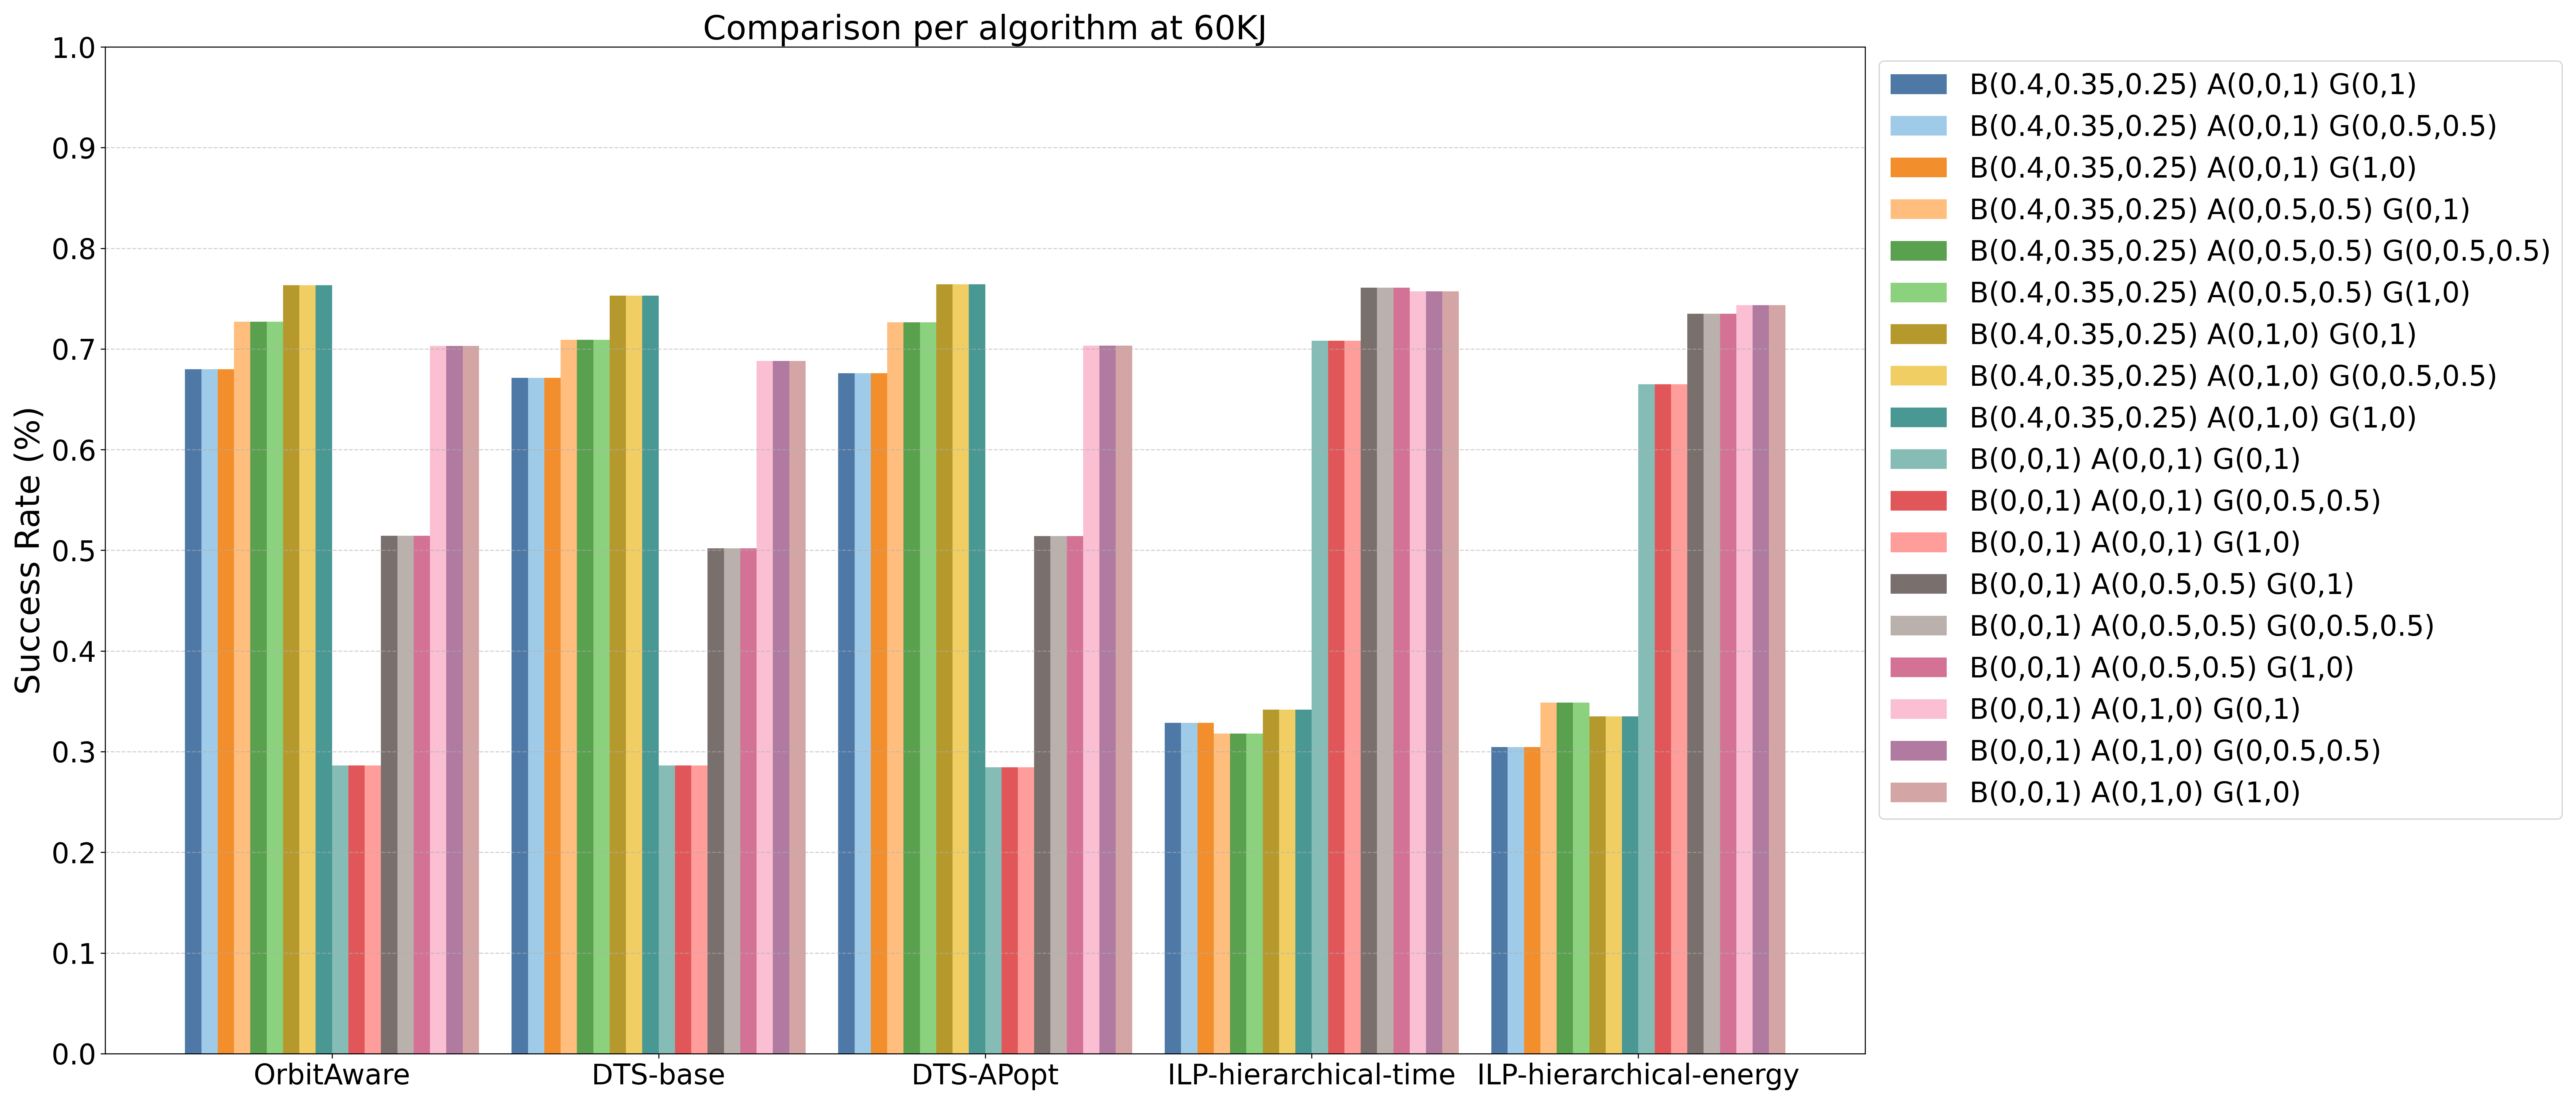
\includegraphics[width=1\paperwidth, height=0.4\textheight, keepaspectratio]{comparison_algos_60000.png} 
    \caption{Confronto algoritmi a 60KJ}
    \label{fig:grafico1}

    \vspace{1cm} % Spazio verticale tra i due grafici (regolalo a piacere)

    % --- SECONDO GRAFICO ---
    \noindent
    \hspace*{-3cm} 
    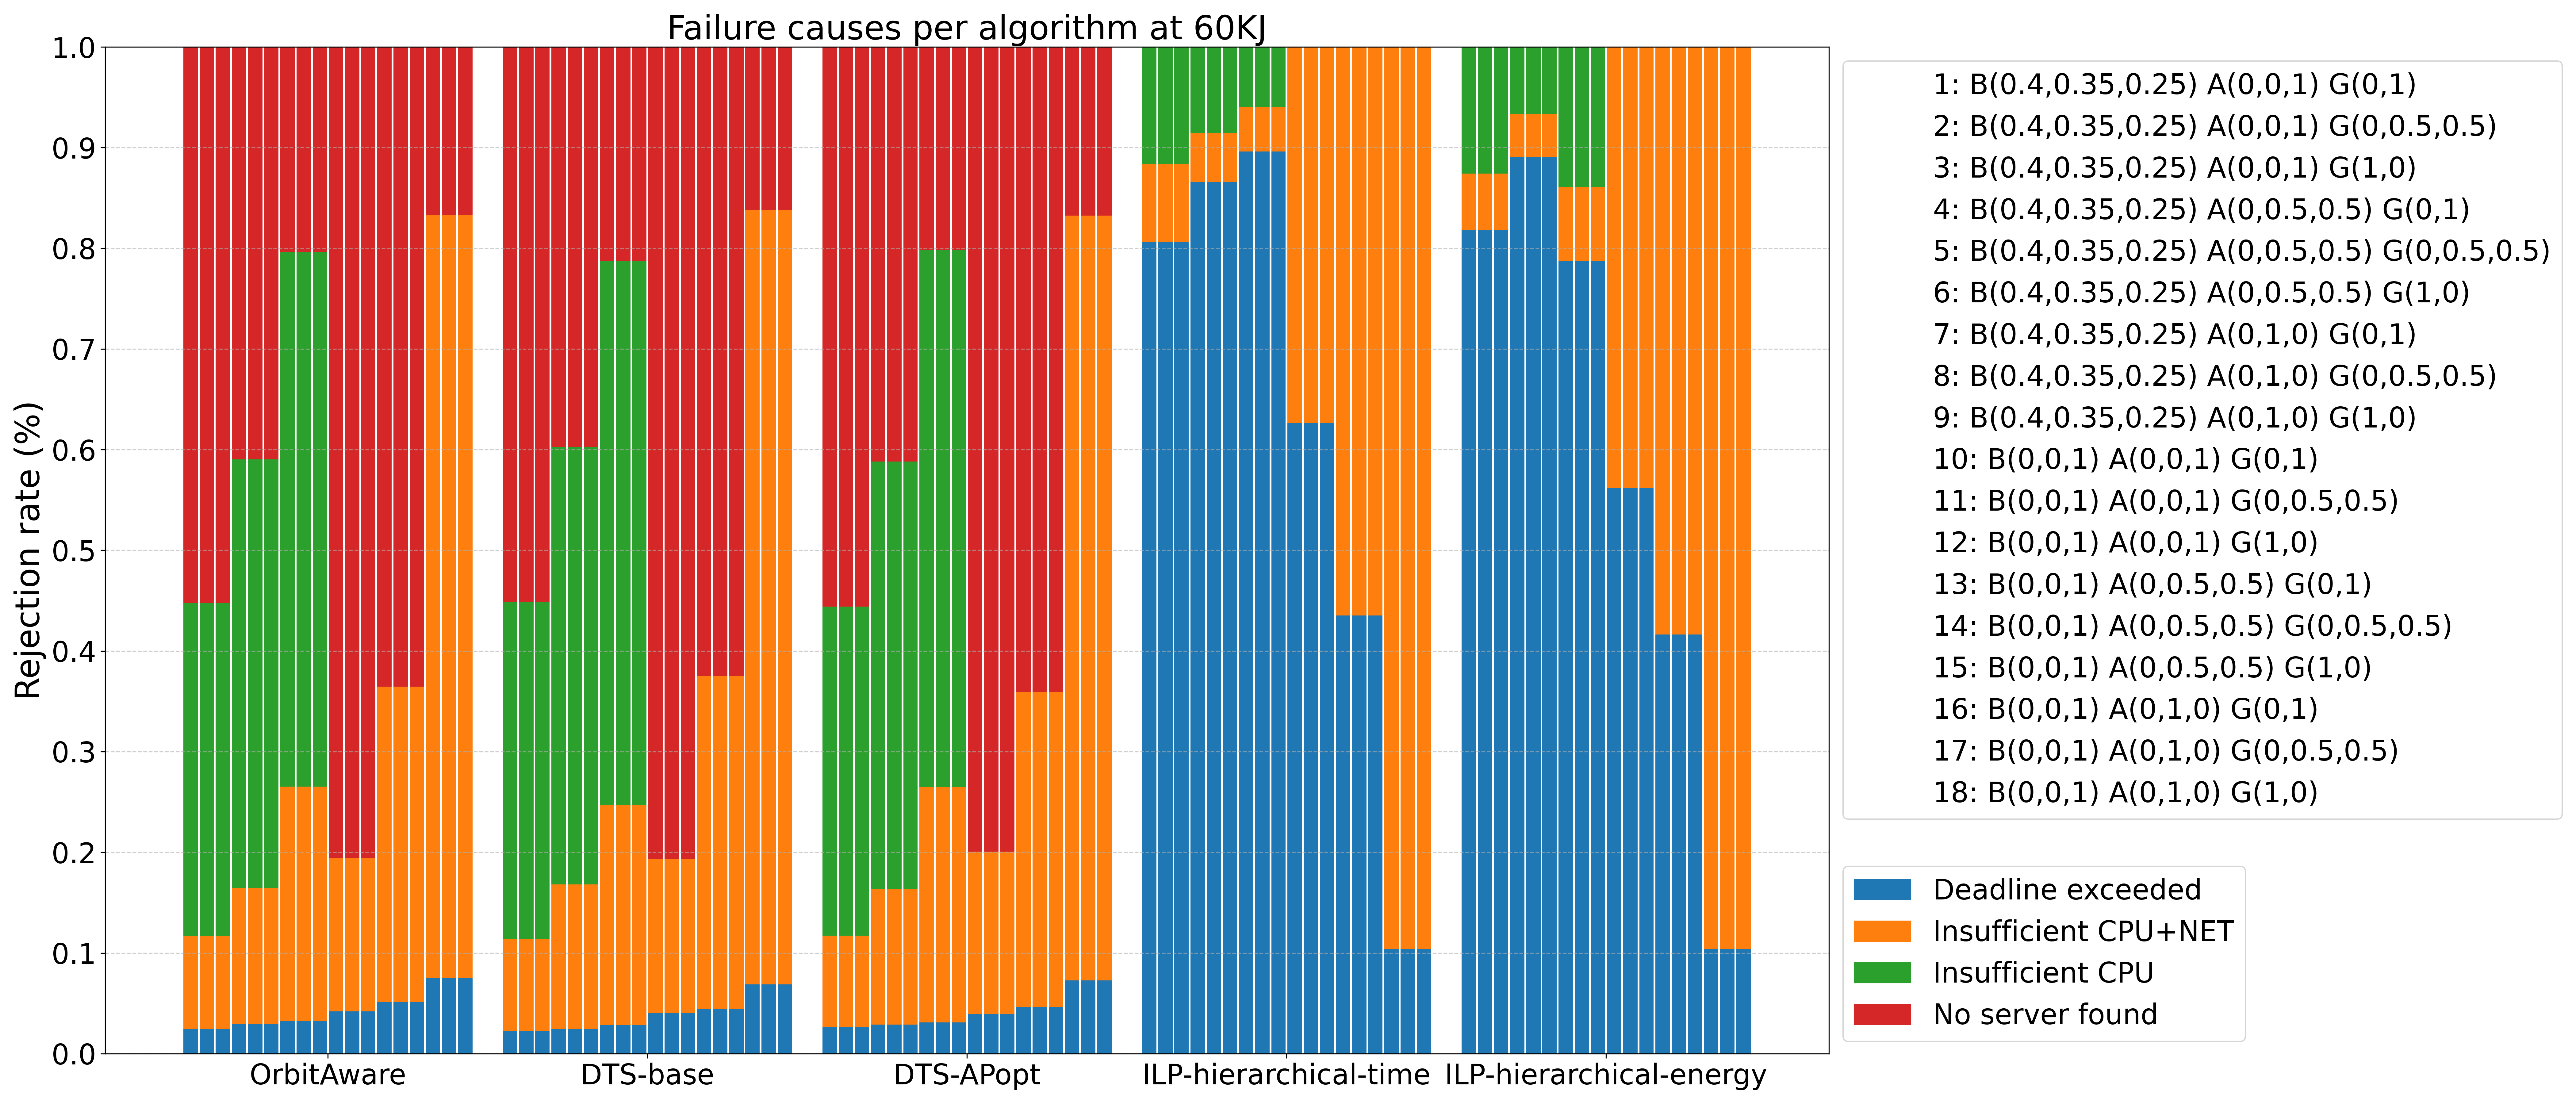
\includegraphics[width=1\paperwidth, height=0.4\textheight, keepaspectratio]{rejection_causes_60000.png} 
    \caption{Confronto rejection causes a 60KJ}
    \label{fig:grafico2}
\end{figure}

\begin{figure}[H] % Forza la posizione 'qui'
    \noindent 
    % --- PRIMO GRAFICO ---
    \hspace*{-3cm} 
    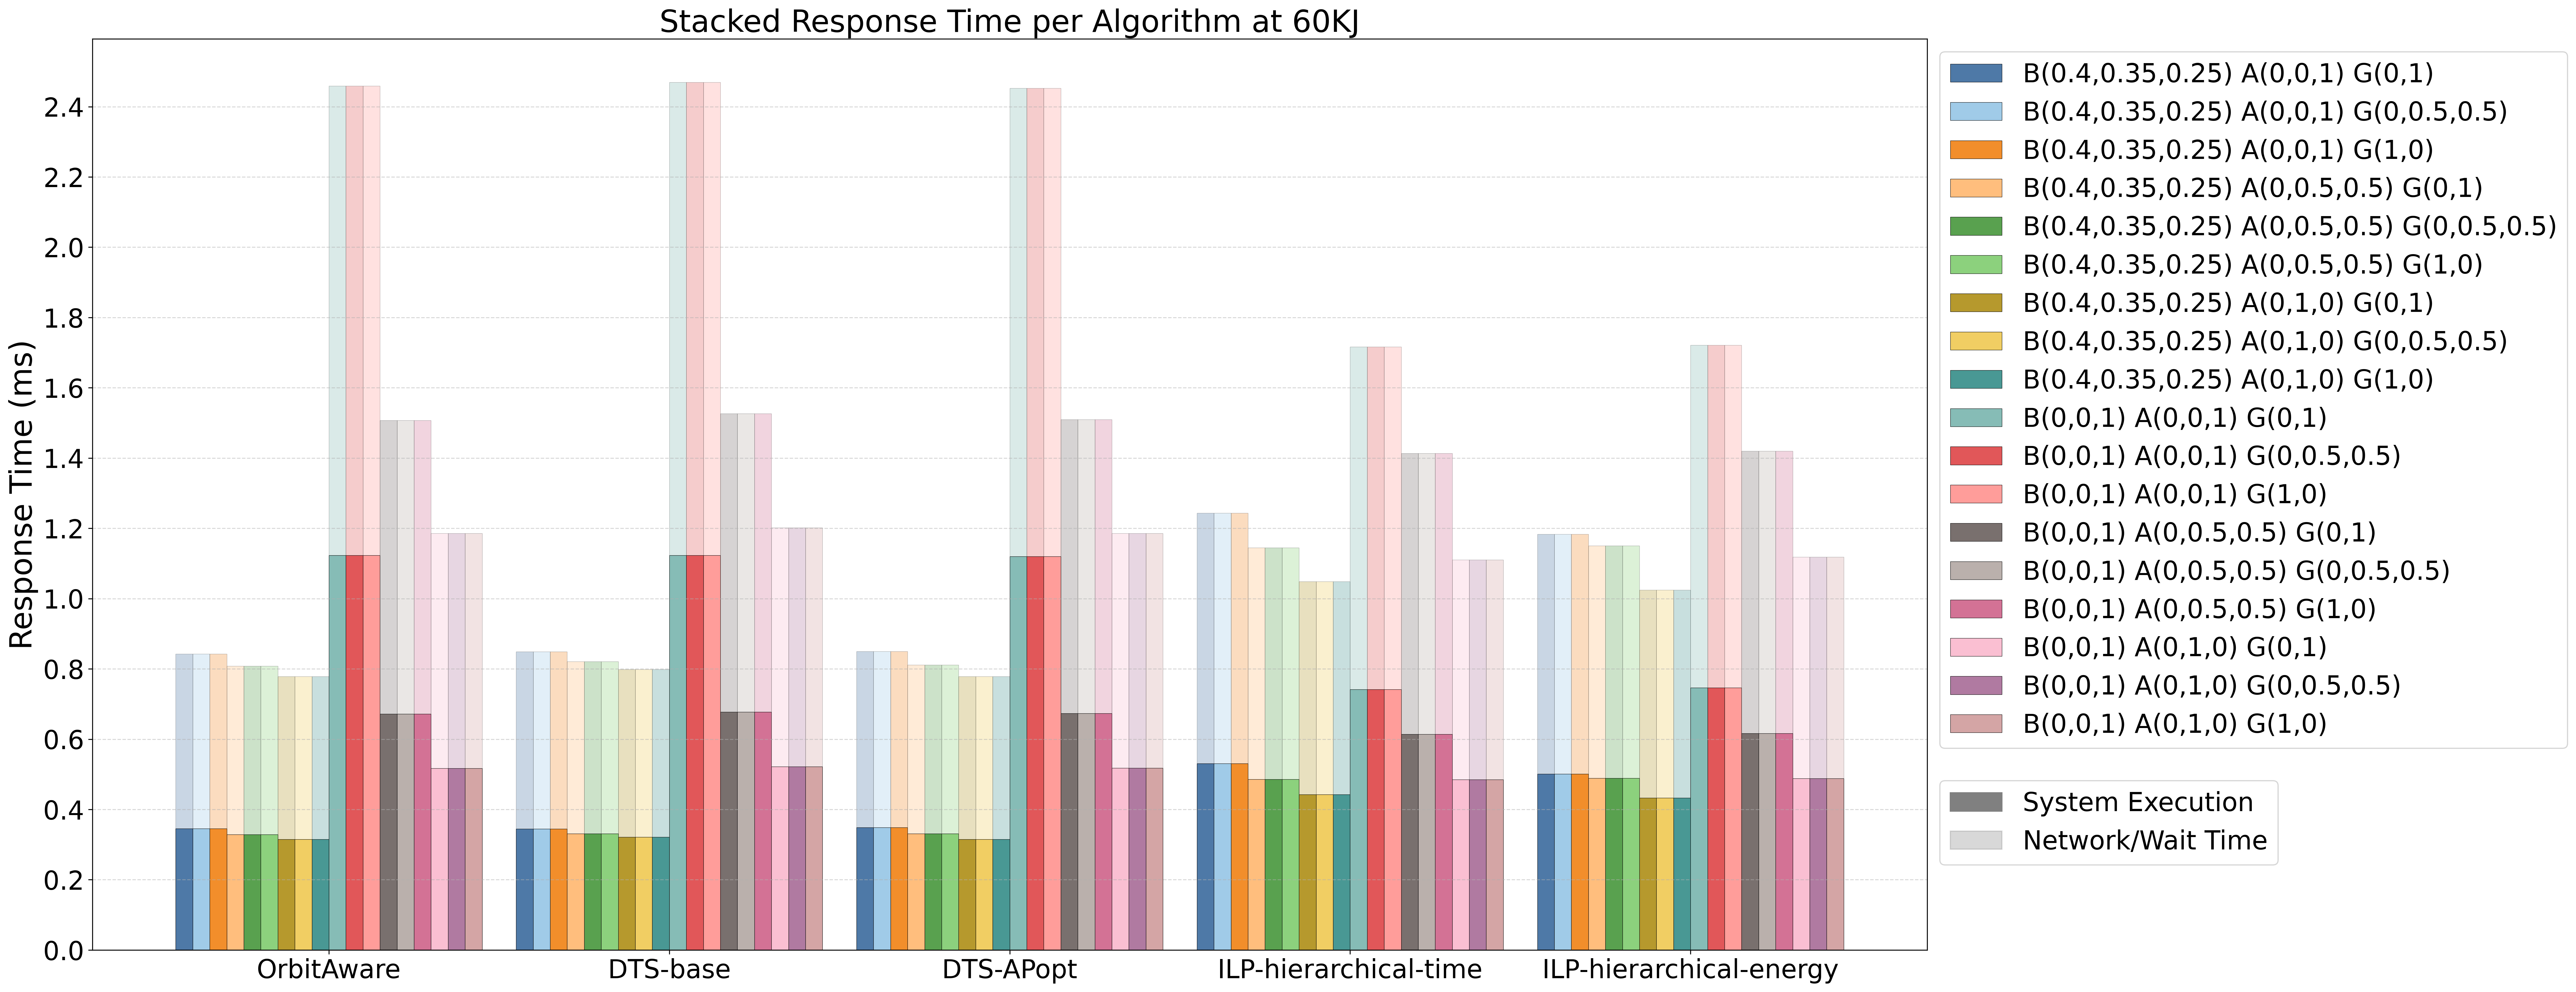
\includegraphics[width=1\paperwidth, height=0.4\textheight, keepaspectratio]{response_time_60000.png} 
    \caption{Confronto response times a 60KJ}
    \label{fig:grafico3}

\end{figure}


\end{document}